\section{振動試験(加藤・飯島)}
衛星は,打ち上げ時・軌道上での過酷な環境に耐えうるよう設計され,それが試験により確認される必要がある.CubeSatのようなピギーバック(相乗り)衛星が打ち上げ環境により破壊もしくは爆発を起こしてしまった場合,その影響は主衛星にも及ぶ.打ち上げ時の環境は2つの振動環境と準静的加速(打ち上げの際の加速)環境によりなる.振動試験では打ち上げ時以上の過酷な加振を行い破壊が発生しないことを確認することで,衛星が打ち上げに耐えうることを示す.\par
本章では振動試験の目的・内容・実施時の注意等をなるべくわかりやすく説明することから,本章が「振動試験初心者マニュアル」となることを期待する.試験実施時の詳細な試験手順及び試験における確認事項は振動試験ハンドブック\cite{vibration_test_handbook}ならびに試験の際の計画書・報告書・手順書\cite{EM_vibration_test_manual}\cite{EM_vibration_test_report}\cite{EM_vibration_test_plan}\cite{FM_vibration_test_manual}\cite{FM_vibration_test_report}\cite{FM_vibration_test_plan}\cite{re_FM_vibration_test_manual}\cite{re_FM_vibration_test_report}\cite{re_FM_vibration_test_plan}を参考にしてほしい.\par
\vspace{\baselineskip}
※ちなみに,僕(加藤)が振動試験場に行って最初に発した言葉は帰り際の「サインバースト試験って何ですか?」である(試験前の下見だったので,僕の知識不足は試験に影響を与えなかったということは一応書いておく).衛星開発をやらなければ日常で振動試験などに出会うはずがない.わからないことが多いのは当然であり,試験場の方やJAXAの方もそれは承知してくれているはず.この文書を読んでいる試験担当者には試験前,試験中に多くの質問をすることを期待する.また,この文書を読んでいるのが担当者の先輩,教員であれば分からないことを率先して質問し,担当者が質問のしやすい空気を作っていただければ幸いである.

\subsection{振動試験とは}
\subsubsection{試験目的}
振動試験の目的は以下の4つである.
\begin{enumerate}
	\item 打ち上げ環境に耐えうることの確認
	\item 剛性の確認(ロケットとの振動連成の防止)
	\item 組み立てに伴う欠陥(ワークマンシップエラー)がないことの確認
	\item 構造数学モデルの確認
\end{enumerate}
打ち上げ時の振動環境以上の加振を行うこと,また固有振動数と伝達関数の値及び試験前後でのそれの変化を調べることにより1,2,3,4を示す.それに加え電気的な機能試験(チャタリング検知・機能試験)も行い1を示す.
また4に関してはモード形状も含めたモードパラメータに対する精度が要求された場合のみモーダルサーベイ試験が必要となる(OrigamiSat-1振動試験ではモーダルサーベイ試験も実施している).

\subsubsection{打ち上げ環境}
%宇宙機に対して実施される振動試験は、打上げ時の振動環境に対する耐性、実機の剛性(最低次固有振動数)、製造・組立上のワークマンシップ、構造数学モデルの妥当性を確認する目的で実施される\cite{vibration_test_handbook}.\par
打ち上げ時の環境は準静的加速環境と振動環境に分かれ,さらに打ち上げ時の振動発生要因は多岐にわたる.また液体ロケットと固体ロケットにおいてもその振動環境は異なる.しかし大別すると打ち上げ時の過酷な環境は
\begin{itemize}
	\item 数Hz~数十Hzの低周波過渡振動:リフトオフ時のブースターの推力立ち上がり,大気中飛行時の乱流,1/2段分離時の分離スプリング力等によるもの
	\item 数百Hz~数千Hzの高周波ランダム振動:エンジン排気流から生じる音響,フェアリング壁の液体加振によるもの
	\item 準静的加速度:ロケット発射時の加速によるもの
\end{itemize}
の2つの振動環境と準静的加速環境の合計3種類となる.\par
%fig:打ち上げシーケンス及び打ち上げ時の主要な振動環境
\begin{figure}[H]
	\centering
	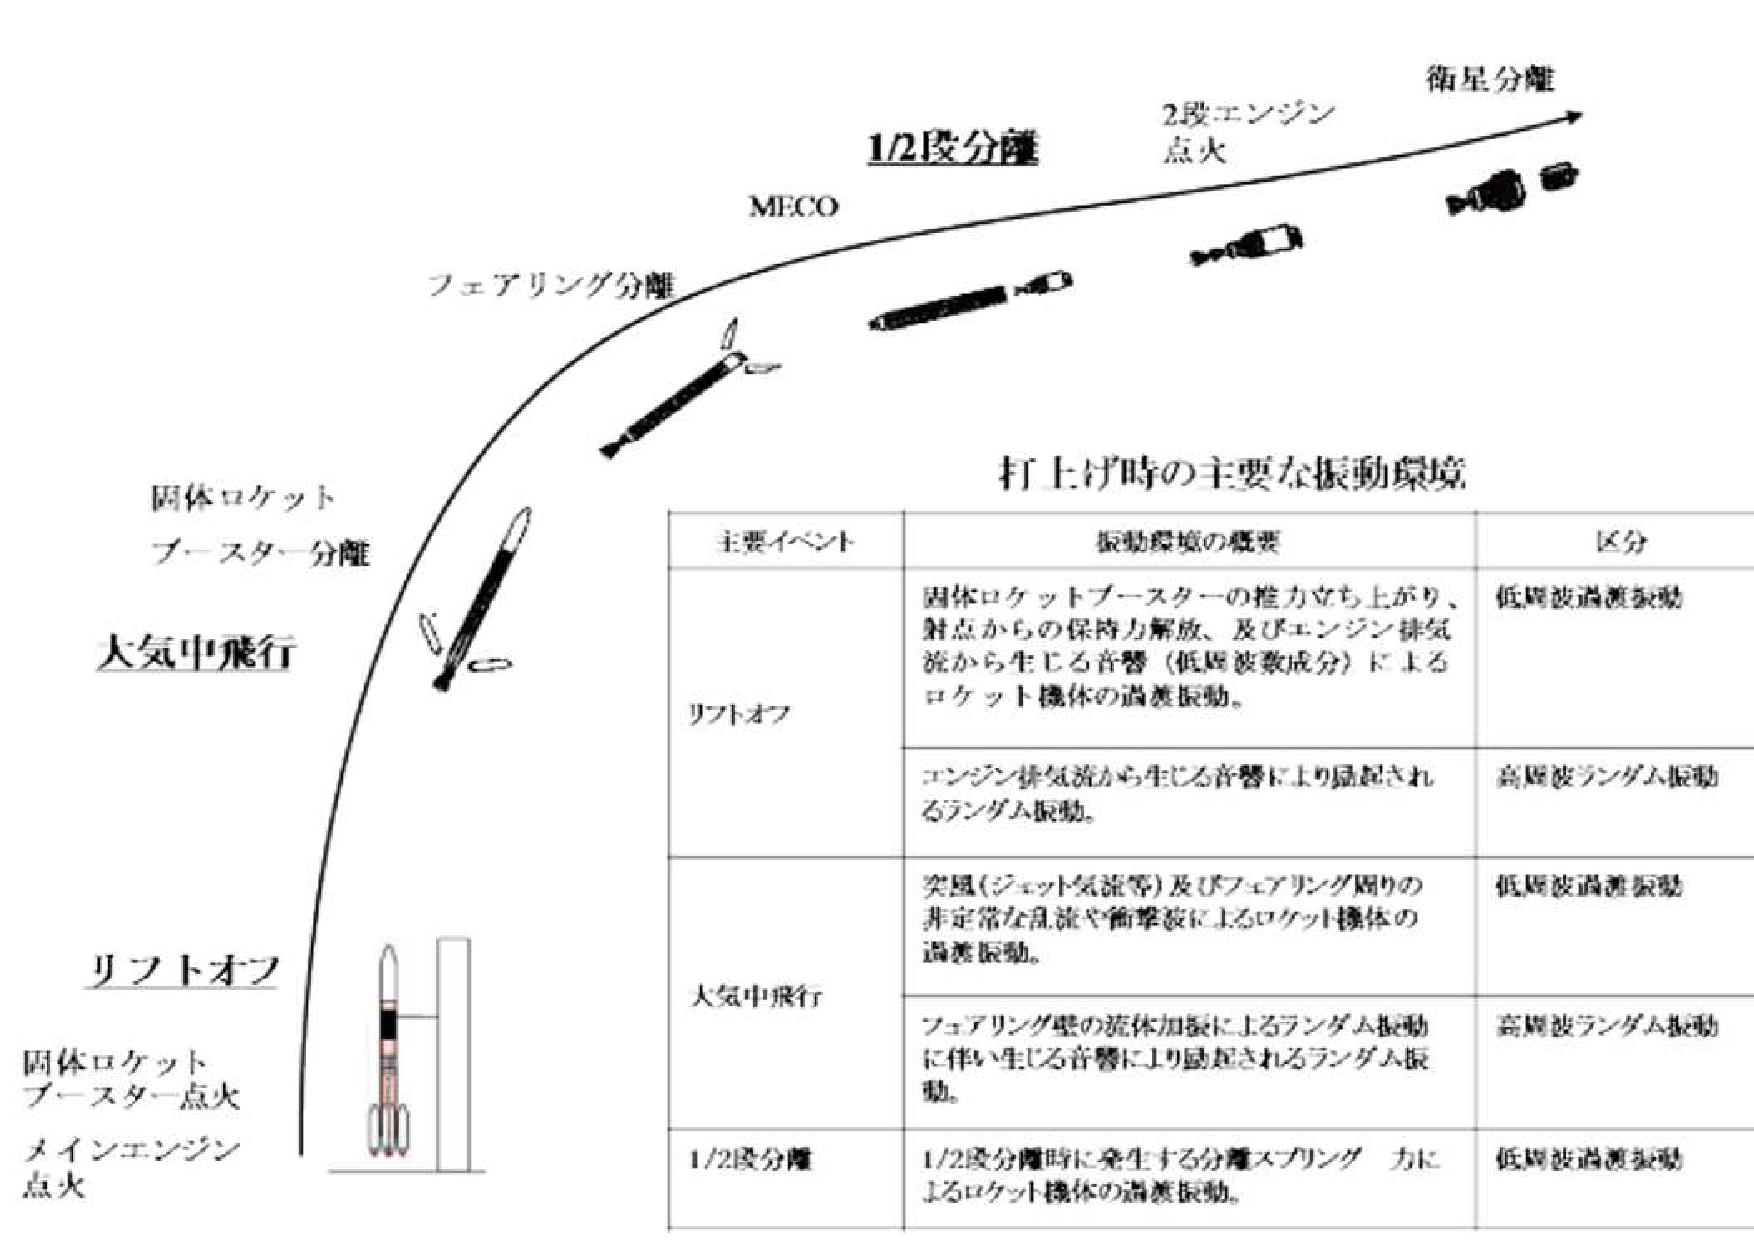
\includegraphics[width=1\linewidth]{04/fig/4-3-1.pdf}
	\caption{打ち上げシーケンス及び打ち上げ時の主要な振動環境\cite{vibration_test_handbook}}
	\label{fig4-3-1}
\end{figure}

\subsection{試験内容}
OrigamiSat-1開発における振動試験においては、上記で示した3種類の環境を模擬した試験にモーダルサーベイ試験(モード形状・固有振動数測定試験)を加えた以下の4種の試験を実施した.

\begin{enumerate}
	\item 正弦波振動試験:低周波過渡振動に耐えうること
	\item ランダム振動試験または音響試験:高周波ランダム振動に耐えうること
	\item サインバースト試験(静荷重試験の代替試験):準静的加速度環境に耐えうること
	\item モーダルサーベイ試験:衛星と振動連成を起こさないこと
\end{enumerate}

%表 2.2-1 振動試験の目的と種類\cite{vibration_test_handbook}
\begin{table}[H]
	\centering
	\caption{振動試験の目的と種類\cite{vibration_test_handbook}}
	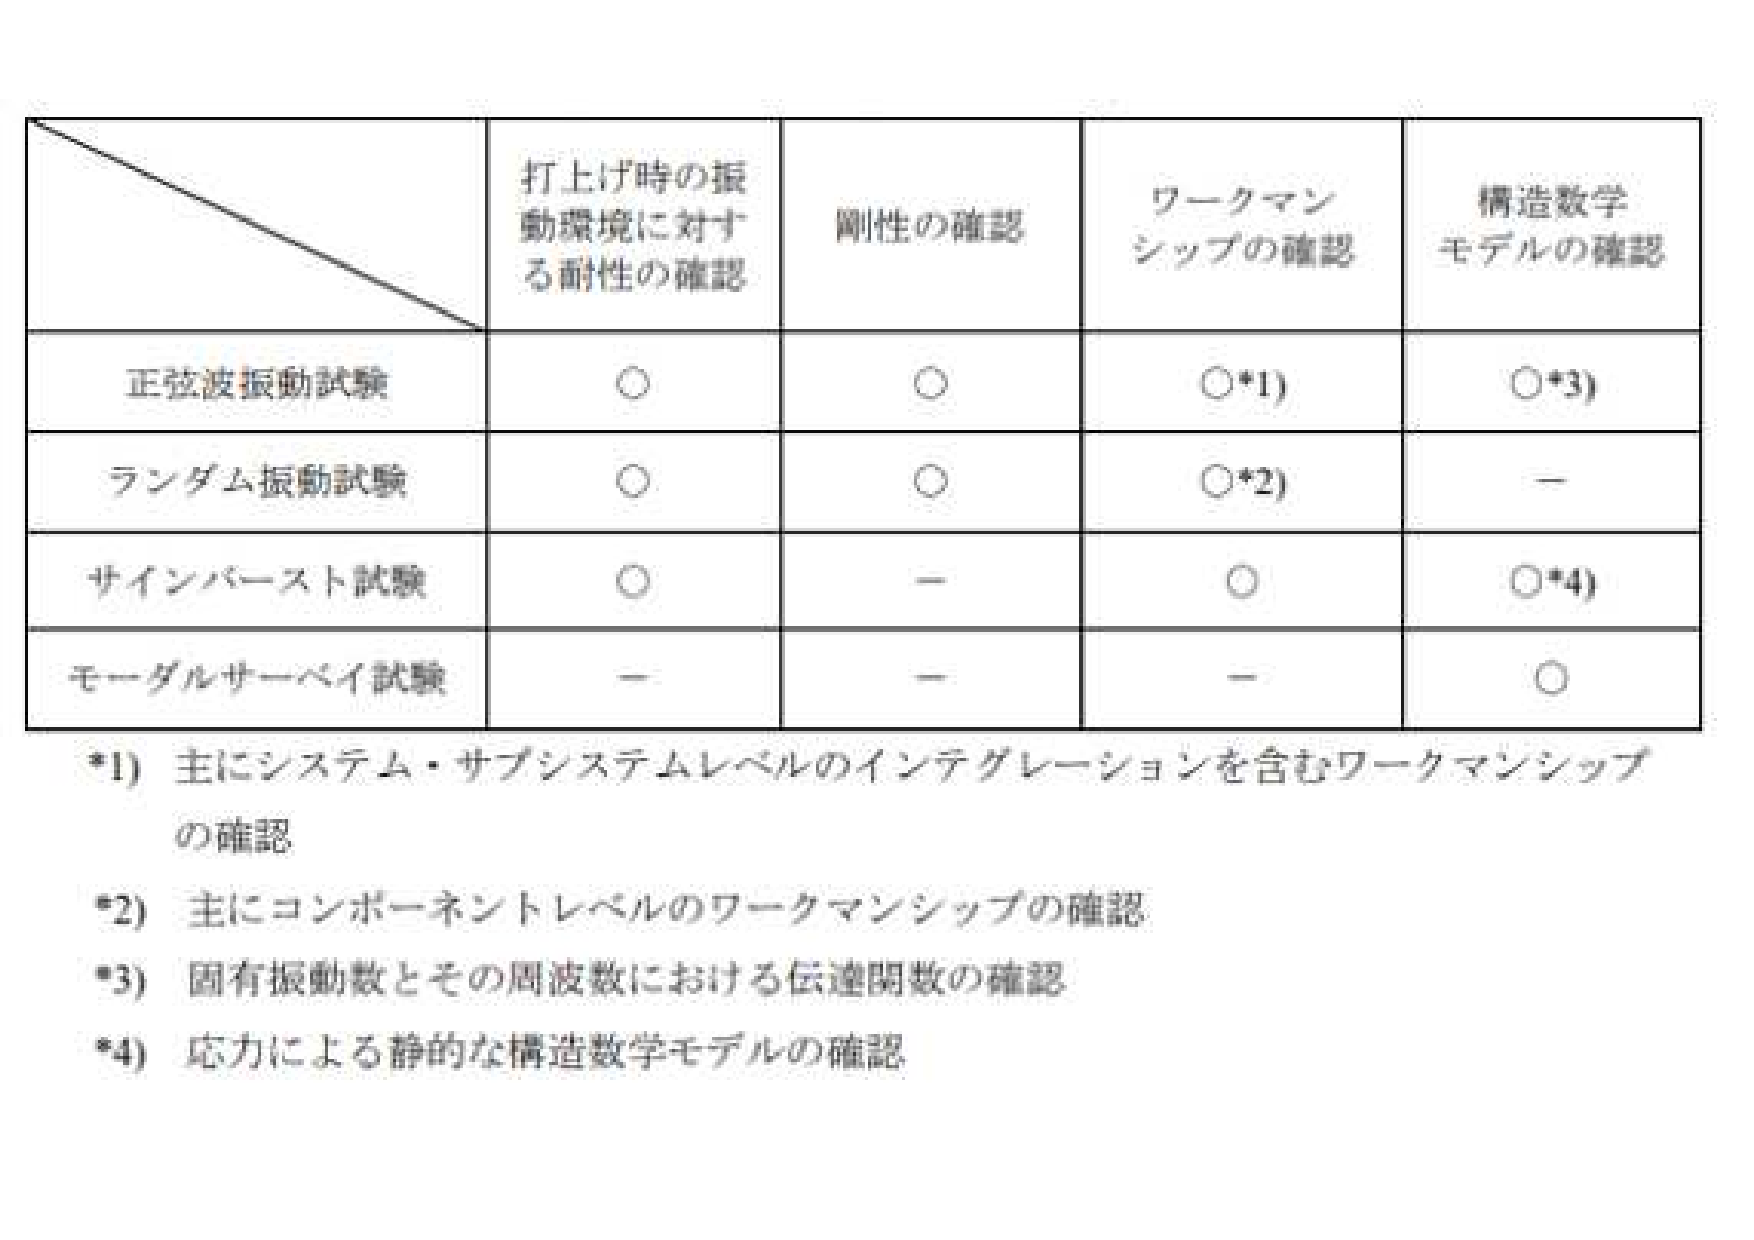
\includegraphics[width=0.9\linewidth]{04/fig/t4-3-2.pdf}
	\label{table4-3-2}
\end{table}


また,試験目的に応じては要求される強さ(AT,Acceptance Test)の加振よりも弱い加振(1/2AT)または強い加振(QT,Qualification Test)を行い,衛星がどの程度の加振に耐えられるのかを確認することもある.EM試験においてはそのような試験も実施した.詳細は後述.

%ここから先,それぞれの加振についてどんな条件で加振すればよいのかを図多めで表す
%どんなことを確認できれば試験としてOkなのかも示す
\subsubsection{モーダルサーベイ試験}
各試験の前後にモーダルサーベイ試験を実施し,その前後でのモード形状および固有振動数に変化がないことを確認する.
試験においては周波数範囲・加速度密度・実効値・時間が指定されているが,公差は指定されていない.
報告書には固有振動数及びモード形状が各試験前後で変化しないことを記載する.変化していた場合は衛星内部で破壊が起こったことが疑われる.

%報告書に載せた図
\begin{figure}[H]
	\centering
	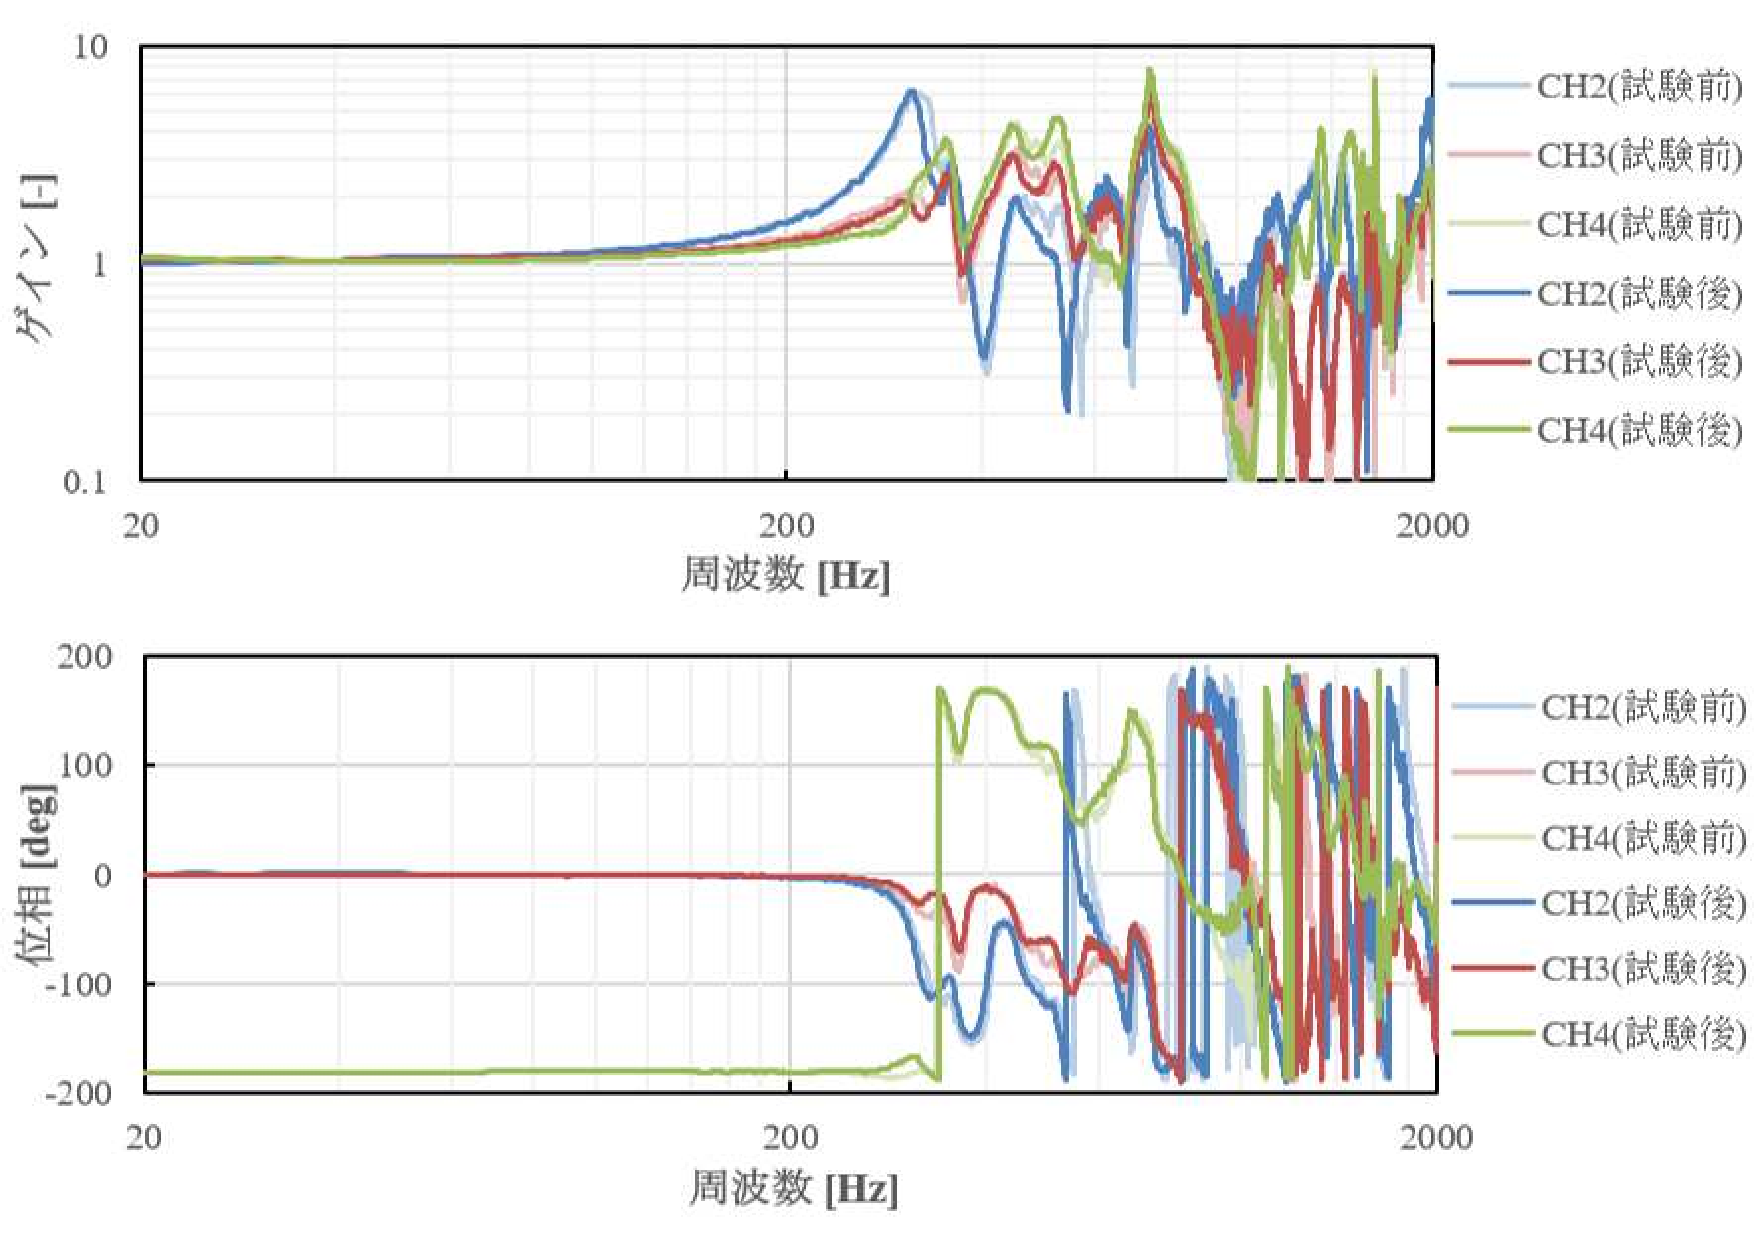
\includegraphics[width=1\linewidth]{04/fig/4-3-3.pdf}
	\caption{FM試験におけるモーダルサーベイ試験結果\cite{FM_vibration_test_report}}
	\label{fig4-3-1}
\end{figure}


\subsubsection{正弦波加振試験}
周波数を変えながら加振を行い低周波過渡振動に耐えうることを確認する.試験は2種類の周波数帯(22-36Hz,43-57Hz)で行った.
試験においては加速度・掃引速度(周波数変化速度)・往復数・公差が指定されている.
報告書には指定された強さの試験ができていることを記載する.

%報告書に載せた図
\begin{figure}[H]
	\centering
	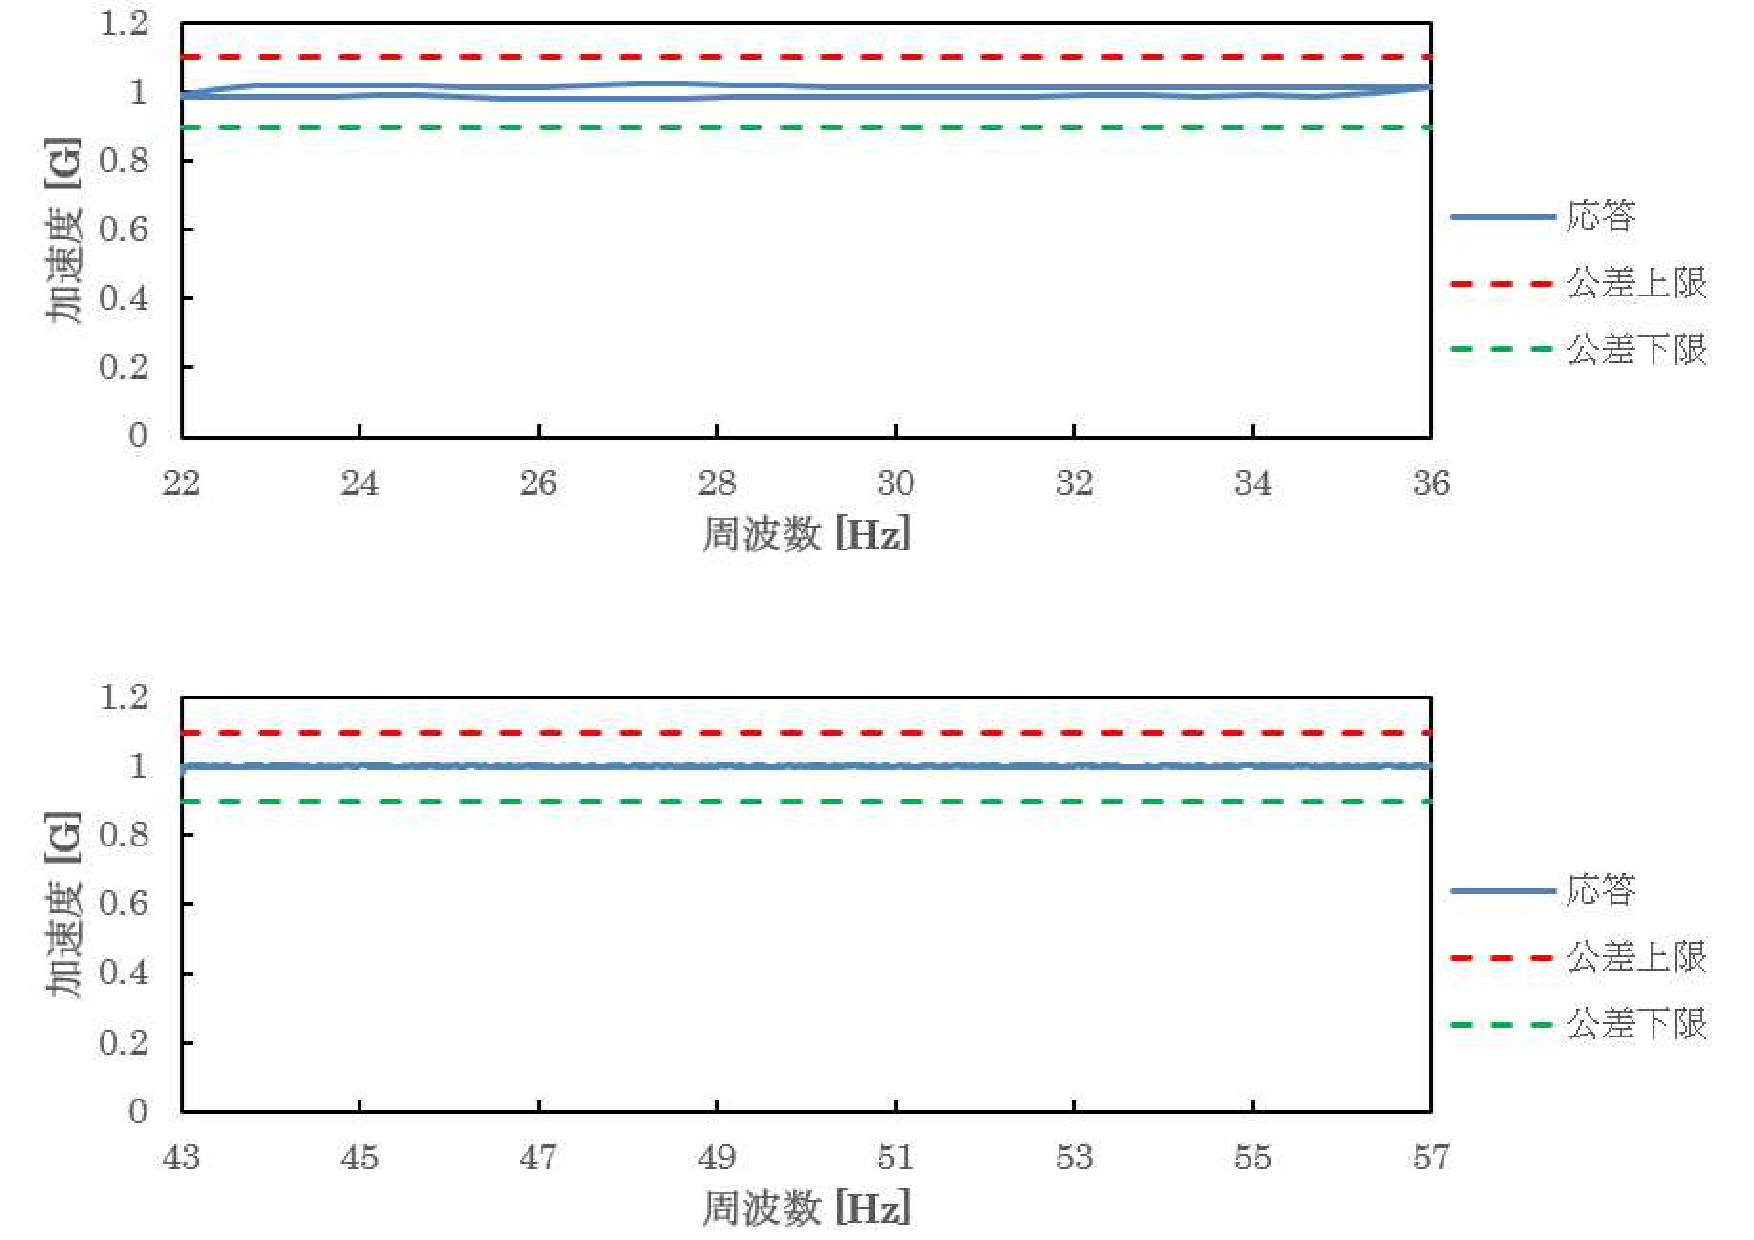
\includegraphics[width=1\linewidth]{04/fig/4-3-4.pdf}
	\caption{FM試験における正弦波加振試験結果\cite{FM_vibration_test_report}}
	\label{fig4-3-1}
\end{figure}


\subsubsection{ランダム振動試験}
ランダムな振動を加え,高周波ランダム振動に耐えうることを確認する.
ランダム振動試験においては周波数範囲・加速度密度・時間・公差が指定されている.
時間は既定の公差内の振動になってから測定し始める.公差内の振動になるまでにかなり時間がかかるが気長に待つ.
報告書には指定された公差内で試験ができていることを記載する.
高周波の範囲(1700Hz前後)で一部だけ公差を外れることがある.試験場で伝達関数を確認してもらえばわかると思うが,高周波の部分は伝達関数が安定しておらず制御のしにくい部分なのでこうなることがある.固有振動数と大きく外れていることを報告書に記述すれば問題ない.

%報告書に載せた図
\begin{figure}[H]
	\centering
	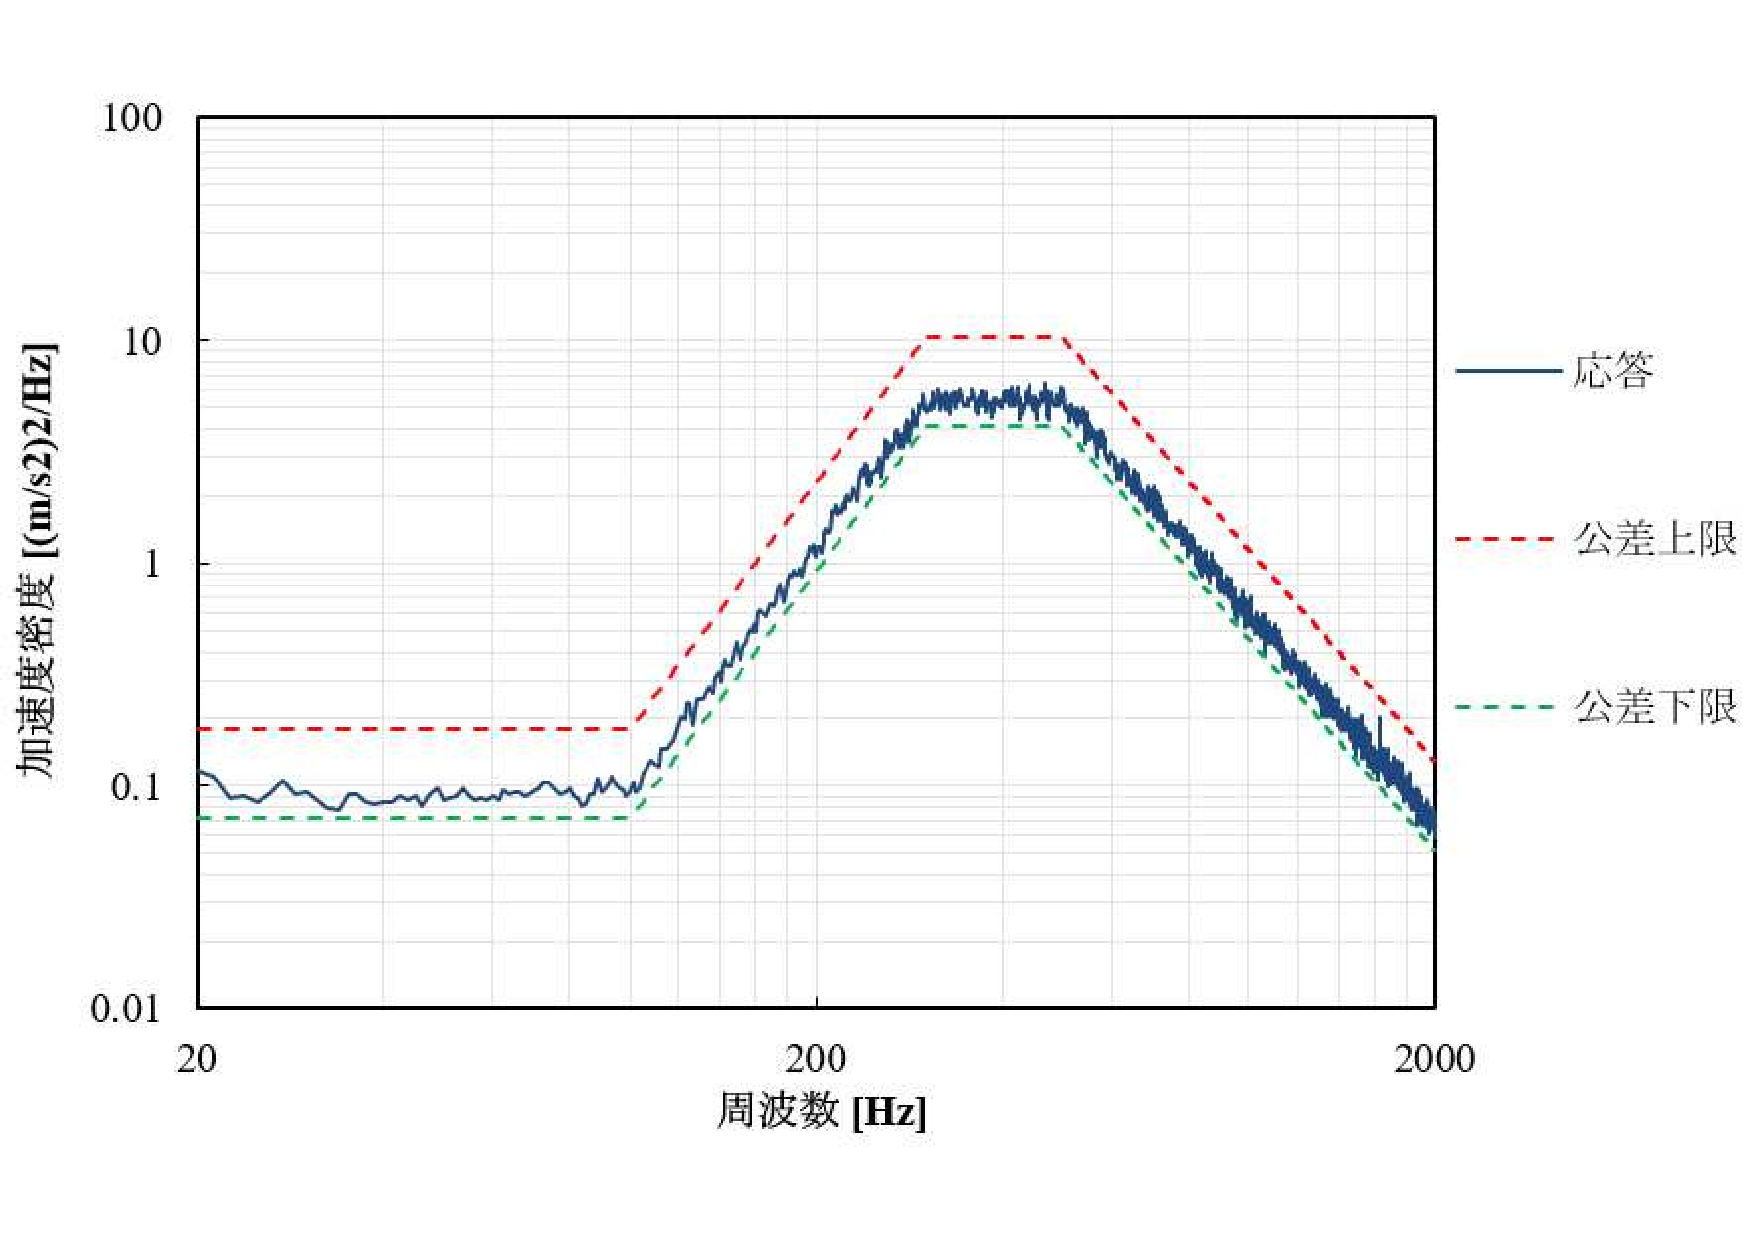
\includegraphics[width=1\linewidth]{04/fig/4-3-5.pdf}
	\caption{FM試験におけるランダム振動試験結果\cite{FM_vibration_test_report}}
	\label{fig4-3-1}
\end{figure}

\subsubsection{サインバースト試験}
サインバースト加振を行い準静的加速度環境に耐えうることを確認する.
サインバースト試験においては周波数・サイクル数(波数)・加速度・公差が指定されている.
この試験は5秒程度で終わる.
報告書には指定された強さの試験ができている(指定された加速度の波が指定された回数観測できている)ことを記載する.


%報告書に載せた図
\begin{figure}[H]
	\centering
	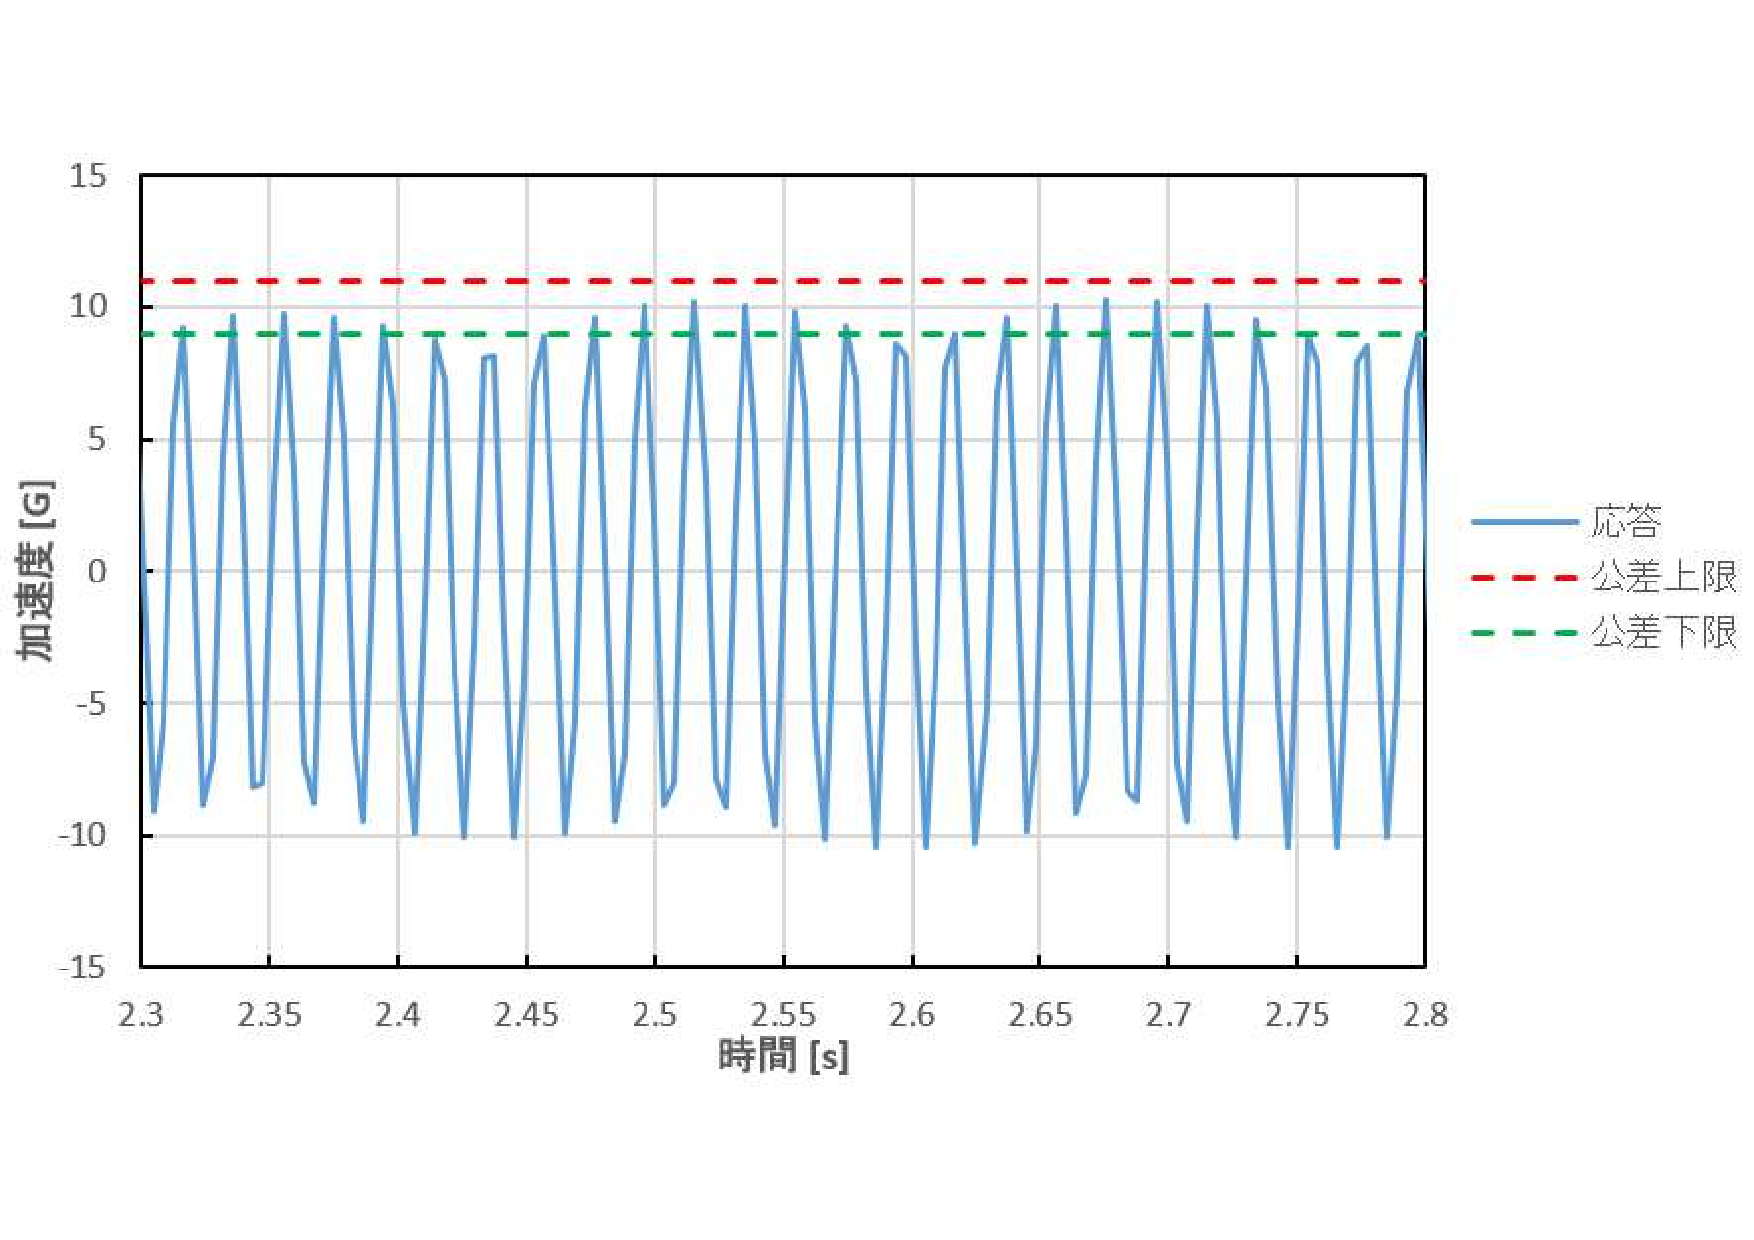
\includegraphics[width=1\linewidth]{04/fig/4-3-6.pdf}
	\caption{FM試験におけるサインバースト試験結果\cite{FM_vibration_test_report}}
	\label{fig4-3-1}
\end{figure}


\subsection{各試験の概要}
\subsubsection{EM振動試験}
2017年12月25-27日に福井県工業技術センターにて実施.
EMにおける振動耐性を確認した.
EM振動試験の目的は次の3点である.(ただし3点目は主要な目的ではない)
\begin{enumerate}
	\item 打ち上げ環境よりも厳しい振動条件(QTレベル)に耐えうることの確認
	\item FM振動試験でATレベルを負荷したときのデータと比較するためのデータを取得
	\item FM振動試験の練習(起こりうるヒューマンエラーを把握し未然に防ぐ)
\end{enumerate}
各試験はATレベルとQTレベルで実施し,ランダム振動試験については上記に加えて1/2ATレベルも実施した.

QTレベルの試験を行うのは目的1のためであり,逆にQTレベルのみがEM試験の必要条件である.
QTレベルは試験条件が厳しいためEMにのみ負荷し,FMには負荷しない.
EM振動試験におけるATレベル試験は目的2のためであり,またQTレベルを負荷する前に異常が出ないことを確認する予備試験の役割も担う.つまり,ATで異常が発生した場合,いきなりQTを負荷して異常が発生した場合よりも被害が抑えられる.
1/2ATレベル試験はATレベル試験の予備試験としての役割のみであり,念の為行う試験である.各試験の中で破壊が起こりやすいとされるランダム振動試験のみ1/2ATレベル試験を行った.

なお,IHIエアロスペース製「CubeSat振動試験用ケース」(イプシロンロケットCubeSat放出装置「E-SSOD」を模した振動試験用ケース)はEM振動試験時には製作中であったため,自作(東工大工場にて加工)したものを使用した.EM振動試験報告書では「E-SSOD代替治具」と呼称.


\subsubsection{FM振動試験}
2019年7月10-12日に宮城県産業技術総合センターにて実施.
EMで確認された振動に対する剛性・モード形状とFMモデルが大きく変わらないこと,FMモデルが要求される振動に耐えられることの確認が目的.
各試験をATレベルのみで実施した.

\subsubsection{FM再振動試験}
2019年9月18-19日に宮城県産業技術総合センターにて実施.
FM振動試験後,CIB基板の取り換えを行った関係から安全審査に関するインヒビットの健全性を確かめるための再試験が必要となった.
ランダム振動試験(ATレベル)とモーダルサーベイ試験のみ実施.

\subsection{振動試験実施の流れ}
本節では,EM/FM/FM再試験を問わず振動試験における全体の流れ(準備→実施→片付け)について記述する.
試験中の細かい確認事項は手順書\cite{FM_vibration_test_plan}等を参考にしてほしい.
また,試験後に見つかった傷がいつからあるものなのかを明確にするために,試験中は写真をとにかく撮りまくること.
%写真を多めにして,イラストで説明.詳しい説明は報告書や計画書を引用しそちらに任せる

\subsubsection{試験場,宿の手配}
%啓さん,ここの部分をお願いします.ここ以外の部分も必要に応じて書き換えてしまっても全く問題ありません.
%また,長くなりそうであれば後ろの不具合,トラブルの節に大変だったこととしてまとめて,そちらを参照という形にしていただいても大丈夫です.


\subsubsection{機能試験}
試験場に到着後,まずはクリーンブースにて衛星の機能確認を行う.
OrigamiSat-1の機能試験では下記のことを確認した.
\begin{itemize}
	\item 放出検知スイッチが正しく機能しており,放出検知スイッチにより電源が遮断されていること(インヒビット健全性の確認).
	\item 各モジュールとOBCの通信の確認
\end{itemize}
振動試験後にも同様の機能確認が必要である.

\subsubsection{衛星のPODへの挿入}
機能確認終了後,衛星をPODへ挿入する.

\subsubsection{加振試験の実施}
%荷物の準備→試験場へ移動→POD挿入→機能確認→加振→機能確認→撤収
試験機の機能確認を行ったのち,衛星をPODごと試験機に固定し,試験を開始する.
試験機の機能確認は衛星をPODに挿入する作業中に実施しておくとスムーズに試験が進む.\par

加振試験中は以下のことを確認する.
\begin{itemize}
	\item 公差内の加振ができていること
	\item 加振試験前後で固有振動数・モード形状に変化が見られないこと
	\item 外部に有意な破損が見られないこと
	\item チャタリング(放出検知スイッチ誤作動)が起きないこと
\end{itemize}

\subsubsection{書類作成}
振動試験前後で以下の書類を作成する必要がある.
\begin{itemize}
	\item 計画書:試験実施2週間前程度
	\item 報告書:試験実施2週間後程度
	\item 手順書:計画書と同じくらいの時期
\end{itemize}
振動試験では,作業は単純だが確認項目が多くまた時間がかかり精神が疲弊しやすい.そのため,手順書(兼チェックリスト)は綿密に作成しヒューマンエラーを未然に防ぐことが重要である.

\subsection{OrigamiSat-1の振動試験において発生した不具合及びトラブル}
本章では,OrigamiSat-1の振動試験において発生した不具合及びトラブルとその対処をまとめる,

\subsubsection{EM試験}
\textbf{側面カメラのレンズ:}
ランダム振動試験中に側面カメラのレンズが外れた.
組み立て時にトルク管理をし忘れ,試験前から緩んだ状態だったためであった.レンズを外した状態で直前のモーダルサーベイ試験からやりなおした.

\subsubsection{FM試験}
%放出検知ピン固着(FM)
\textbf{放出検知ピン固着:}\par
FM試験の後,放出検知ピンが固着しており放出が検知できない状態になっていたことが分かった.
そのあとの放出検知ピン改修の経緯についてはサブシステム開発における構体系の節に詳細をまとめる.

%POD逆(FM)
\textbf{PODの挿入方向を変更:}
POD内挿入口付近に一部にレールがない部分があった.OrigamiSat-1の幕展開部にもレールがない部分があるため,OrigamiSat-1の1/3程度がレールのない部分になってしまうため挿入方向を逆にすることが必要になった.
\begin{figure}[H]
	\centering
	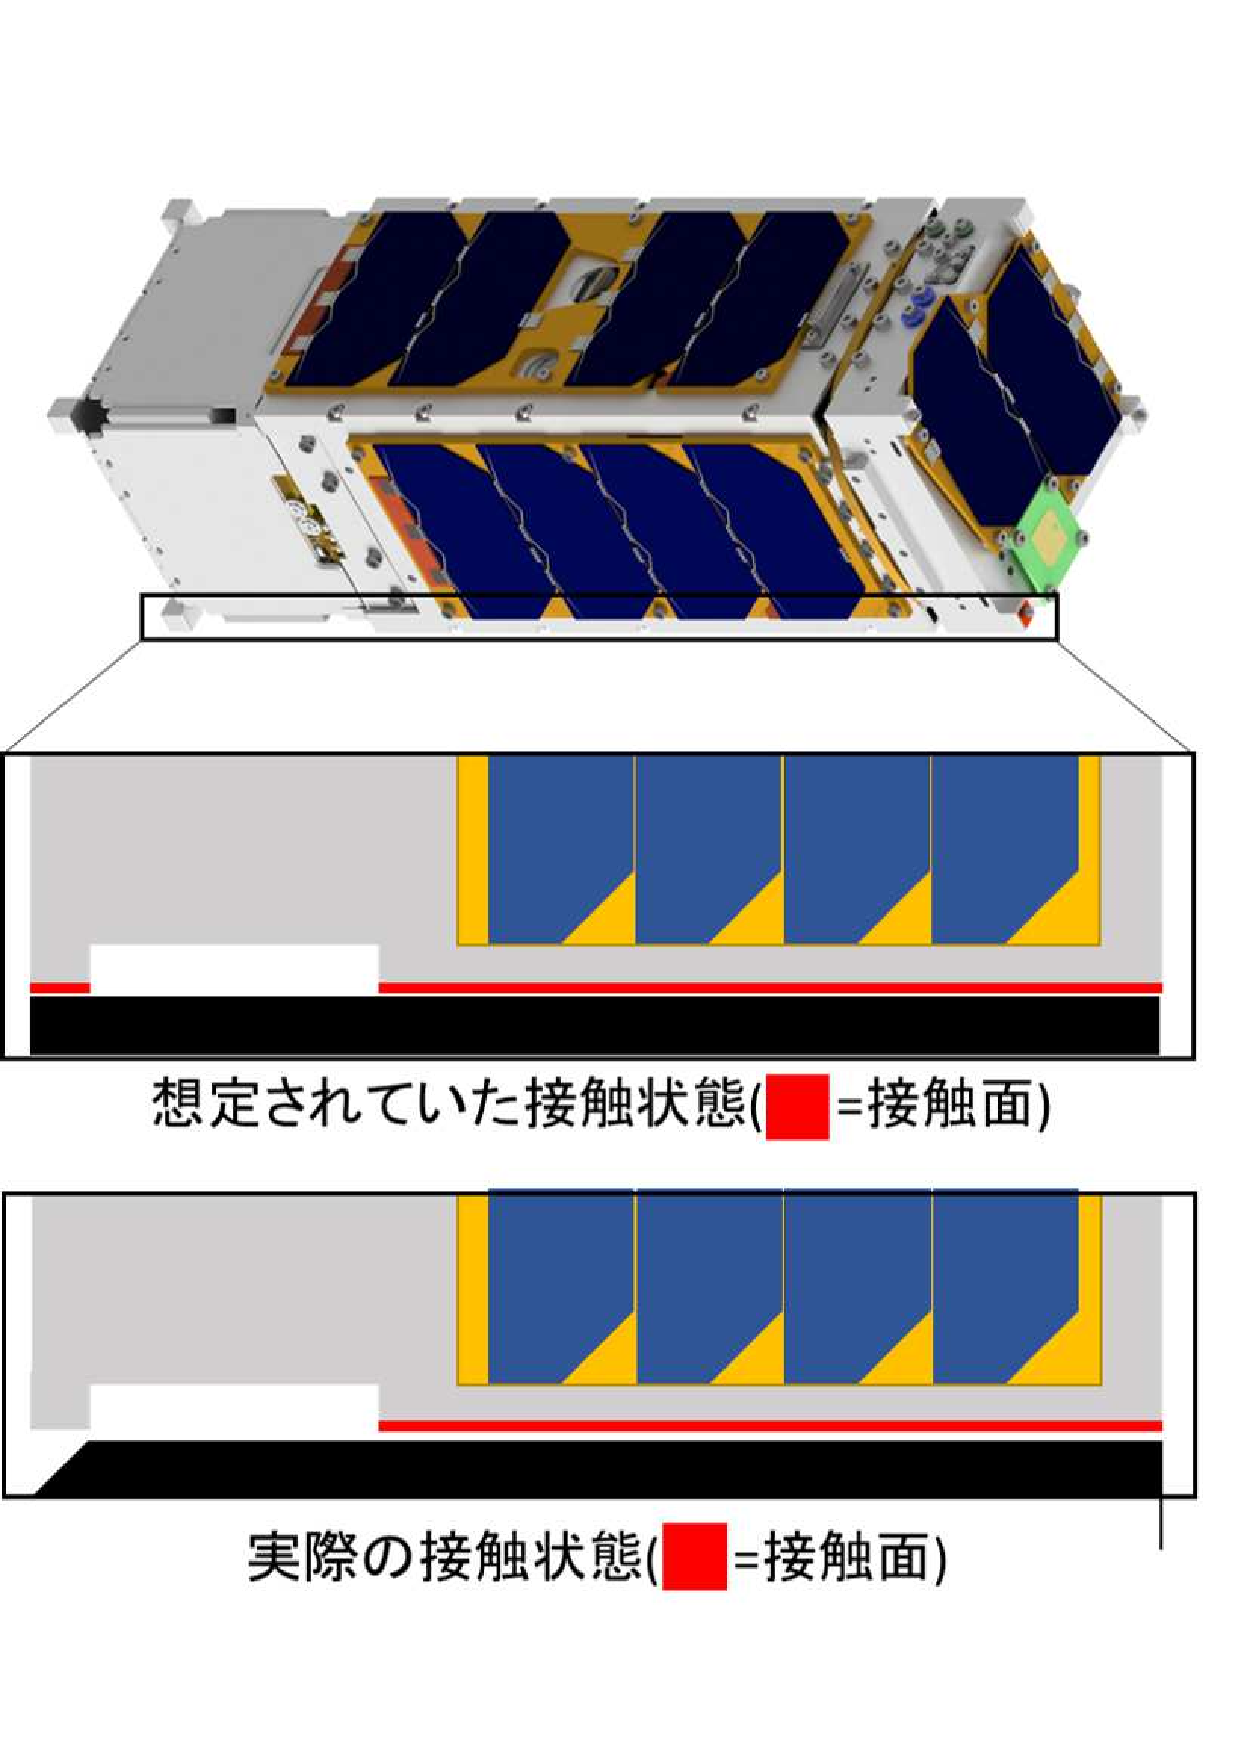
\includegraphics[width=0.7\linewidth]{04/fig/4-3-7.pdf}
	\caption{OrigamiSat-1とPODの接触面}
	\label{fig4-3-1}
\end{figure}



%衛星の電源つけっぱで帰った事件
\textbf{衛星の電源の消し忘れ:}
1日目作業終了後,衛星の電源を落とさずに帰ったため2日目の衛星の電圧が下がった状態で試験を実施した.バッテリの充放電特性も同時に計測しているため,主にそちらに影響が及んだ.

\subsubsection{FM再試験}
チャタリング検知基板に不具合が生じた.現場にいるメンバーでは対応ができず,池谷さんに東京からわざわざ来てもらい対応していただいた.池谷さんありがとうございました.

